\section{Summary}

The study focused heavily on the seeding and navigation mechanisms of the proposed robot system. Minding more on the former, the factors governing on testing the system’s reliability were its row completion time and the number of successfully-filled holes done by itself. In order to quantify the success of filling row holes, a parameter called success rate was used to contrast the holes that were unfilled; which was the ratio of the successfully-filled holes and the total number of holes. The process was trialed 20 times.

As for the navigation mechanism, the current extent of the robot system had managed to be wirelessly controlled through the RaspberryPi microprocessor. The interface for its control was implemented through a local area network that allowed a common point of connection between a laptop (which provided the controls for the system) and the microprocessor (which was being controlled). The alternation of actuating the seeding mechanism and the forwarding the robot was done in such particular manner.

\begin{figure}[h]
	\centering
		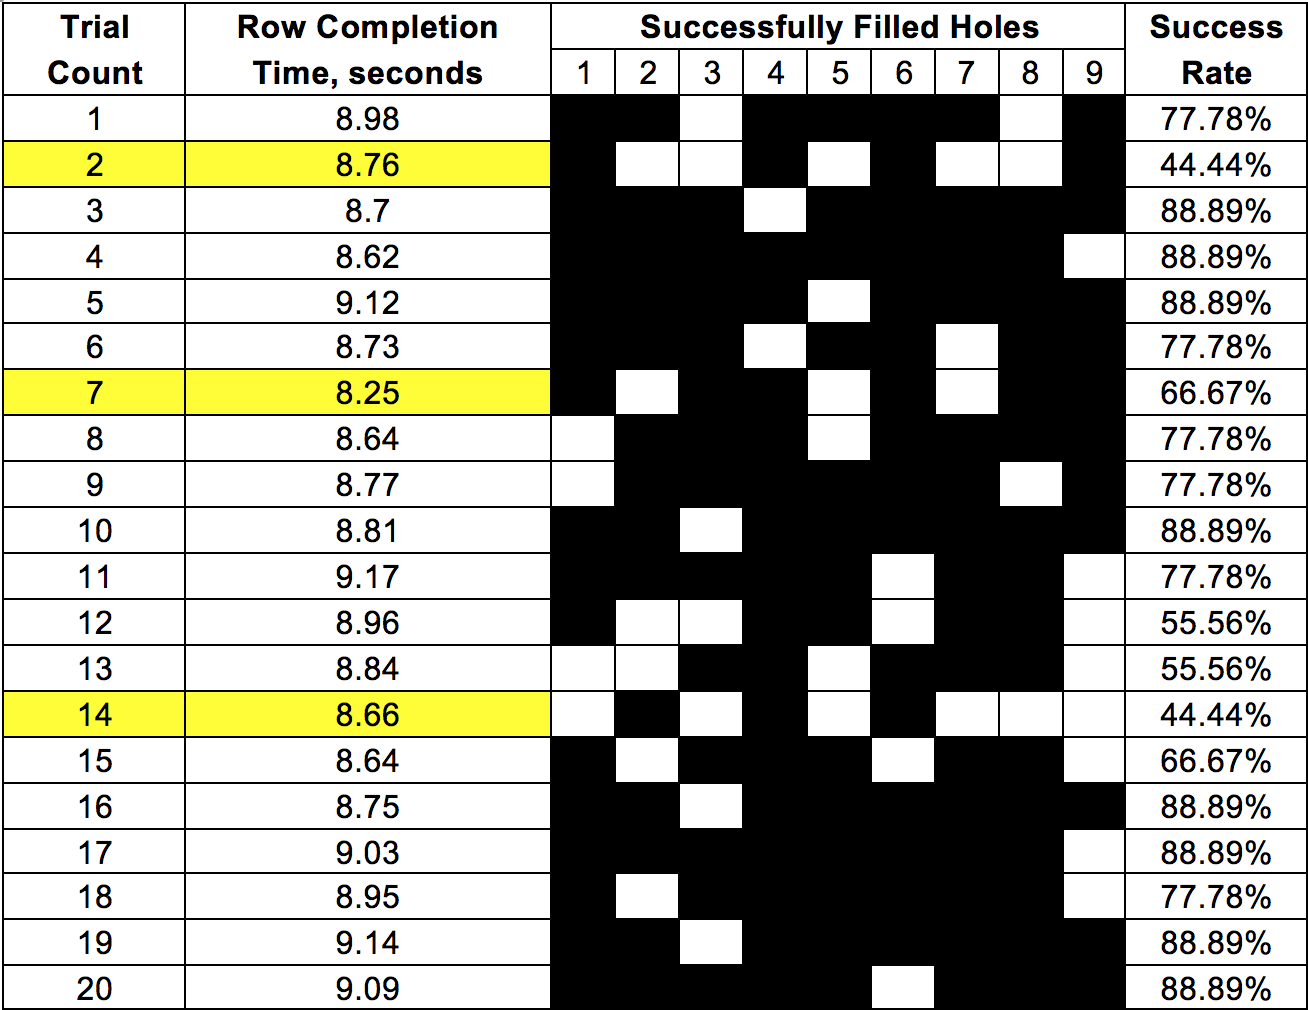
\includegraphics[width=0.5\textwidth]{DAT3}
	\caption{Gantt Chart Analysis of Row Completion Time and Success Rate }
	\label{fig:DAT3}
\end{figure}

Figure~\ref{fig:DAT3} showed the Gantt chart relationship of the time taken by the robot to traverse a row and the number of successfully-filled holes. Visually, the highlighted trials signified the recurring problem of the system: the jamming of the seeding mechanism caused by the seeds being stuck in the crevices of the prototype. The trend was observed that jamming could be anticipated to occur when the number of successfully-filled holes began to decrease significantly; apart from the actual observation of hearing the motor to falter.

\begin{figure}[h]
	\centering
		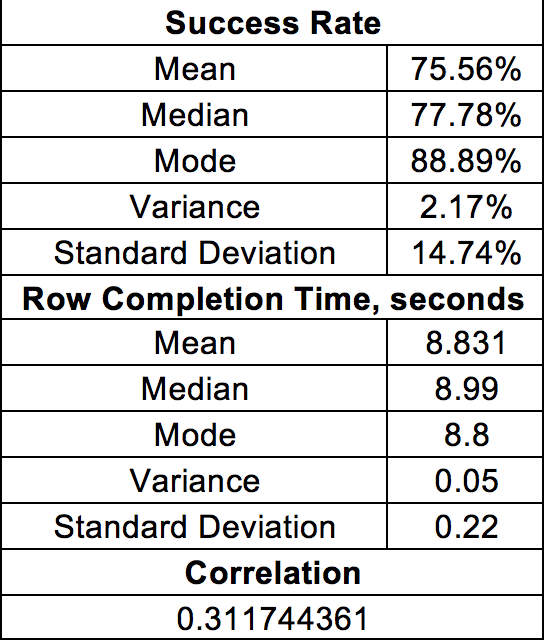
\includegraphics[width=0.5\textwidth]{DAT1}
	\caption{Statistical Analyses of Time and Success Rates }
	\label{fig:DAT1}
\end{figure}

With this set of data, the relationship between the time and success rate was tested through measuring the central tendencies, variances, correlation and regression. For the success rate, it was shown that the mean met the median by a factor of approximately two percent. And, to show consistency of the system, the mode converged to reflecting 88.89\% success rate. With the variance of 2.17\% and standard deviation of 14.74\%, these went to show that the values considerably were close to the average; proving well of its reliability.

The row completion time showed greater performance. The three central tendencies were approximately converging to 8.8 seconds. For convenience, the inspection for the mode was done by rounding-off values of time in one decimal place. The variance and standard deviation of this parameter proved well of both the consistency and reliability of the system. With 0.05 seconds of variance and 0.22 seconds of standard deviation, 20 trials of the system described its performance with the approximations from all the benchmarks aforementioned.

\begin{figure}[!htbp]
	\centering
		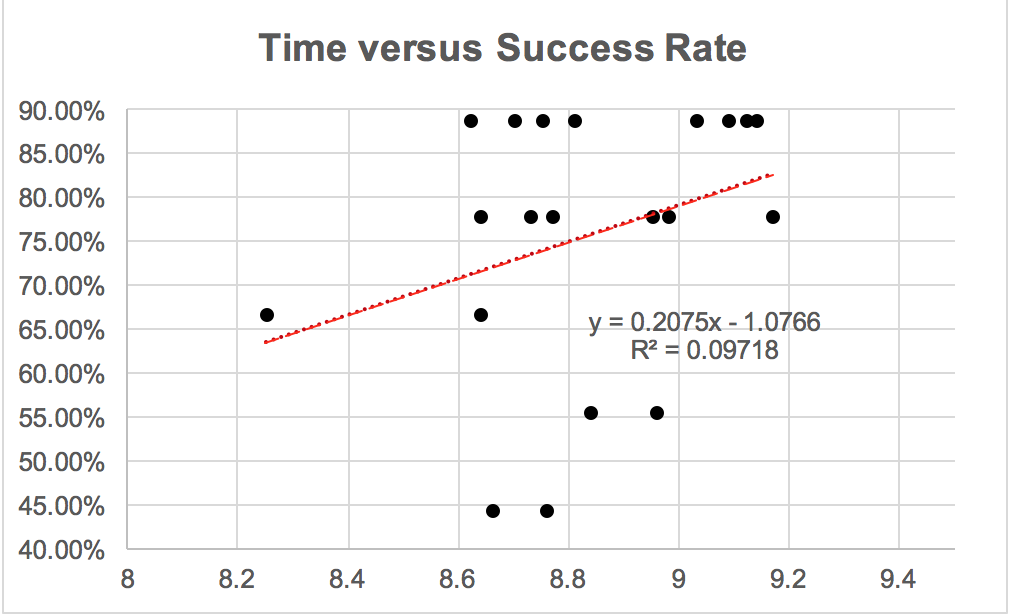
\includegraphics[width=2.5 in]{DAT2}
	\caption{Time versus Success }
	\label{fig:DAT2}
\end{figure}

From the figure~\ref{fig:DAT2}, it illustrated the scatter plot diagram of the system results under 20 trials. A trend line was modeled to estimate the regression analysis of the trial results. Reiterating the value of correlation (~0.3117), it verified that there was a moderate, positive relationship of the time and the success rate. With the coefficient of determination (0.09718), it showed the probability of having independence between the success rate and the time and its difficulty to be predicted by the trend line.